%\documentclass[reprint,amsmath,amssymb,aps,twoside]{revtex4-2} % for editor use only

% For initial submission use these lines
\documentclass[amsmath,amssymb,aps, endfloats, linenumbers]{revtex4-2}



% DO NOT CHANGE THINGS BELOW HERE
\usepackage{graphicx}
\usepackage{amsmath,amssymb,amsfonts}
\usepackage{dcolumn}
\usepackage{bm}
\usepackage{siunitx}
%\usepackage{tikz,pgfplots}
\sisetup{separate-uncertainty=true, multi-part-units=single}
\usepackage[colorlinks,allcolors=blue]{hyperref}
\usepackage{cleveref}
\crefname{equation}{}{}
\crefname{figure}{Fig.}{Figs.}
\crefname{table}{Table}{Tables}
\usepackage{svg}
\svgpath{{./figures}}

% AUTHORS EDIT THIS PART
\hypersetup{%
pdftitle={The Effect of Popper Design on Maximum Jump Height}, % full title here
pdfauthor={Kaitlin Coulanges, Saanvi Dakwale, Samantha Hein, Reese Wallace, and Sashank Yellapragada}, % full author list here
}

\usepackage{fancyhdr}
\pagestyle{fancy}
\fancyhf{}
\fancyhead[RE,RO]{J S\&E \textbf{2}, xx--xx (2026)} 
\fancyhead[LO]{Yellapragada \emph{et al}} 
\fancyhead[LE]{The Effect of Popper Design on Maximum Jump Height} 
\fancyfoot[C]{\thepage}
\fancypagestyle{mytitlepage}{
\fancyhf{}
\fancyhead[C]{Journal of Science \& Engineering \textbf{2}, xx--xx (2026)} % FOR EDITOR ONLY
\fancyfoot[C]{\thepage}
}
\begin{document}

% AUTHORS EDIT THIS PART
\title{The Effect of Popper Design on Maximum Jump Height}

\author{Kaitlin Coulanges}
\author{Saanvi Dakwale}
\author{Samantha Hein}
\author{Reese Wallace}
\author{Sashank Yellapragada}
\email{Contact author: 427syellapragada@frhsd.com} % Replace with the lead contact's email

\affiliation{Science \& Engineering Magnet Program, \href{https://manalapan.frhsd.com/}{Manalapan High School}, Englishtown, NJ 07726 USA}
\date{\today}

\begin{abstract}
This experiment investigates whether the facial expression of a popper affects its maximum jump height using principles of energy conservation. Five ``happy'' poppers and five ``sad'' poppers were compressed to maximum depth and released, converting elastic potential energy into kinetic energy, and then gravitational potential energy. At peak height, mean GPE for happy poppers was \num{96.2 \pm 15.6} \unit{\milli\joule} and for sad poppers was \num{83.1 \pm 9.2} \unit{\milli\joule}. A two-sample, two-tailed $t$-test revealed no statistically significant difference in peak heights ($p = 0.24 > \alpha = 0.05$), or in masses ($p = 0.12 > \alpha = 0.05$). These results support our hypothesis that facial expression does not have any meaningful effect on energy transfer efficiency, and is dictated mainly by elastic properties.
\end{abstract}

\keywords{kinematics, energy conservation, elastic potential energy, poppers}

\maketitle\thispagestyle{mytitlepage}
\section{Introduction}
When a popper is compressed, work is done to deform the material, storing elastic potential energy. This energy can be expressed as: 
\begin{equation}
U_s = \frac{1}{2}kx^2 
\label{eq:epe}
\end{equation}
where $k$ is the spring constant and $x$ is the compression distance \cite{tipler}. Upon release, this stored elastic potential energy is rapidly converted into kinetic energy ($K$), given by:
\begin{equation}
K = \frac{1}{2}mv^2 
\label{eq:ke}
\end{equation}
where $m$ is the mass and $v$ is the velocity \cite{tipler}. As the popper rises, its kinetic energy is transformed into gravitational potential energy (GPE) and represented by the symbol $U_g$. At the maximum height ($h$), the popper’s velocity is approximately zero, meaning the energy is momentarily stored as $U_g$, described as: 
\begin{equation}
U_g = mgh
\label{eq:gpe}
\end{equation}
where $g$ is the acceleration due to gravity \cite{tipler}.

By measuring the maximum height reached, one can estimate the efficiency of this energy transfer. Theoretically, a greater maximum height indicates a greater conversion of elastic potential energy into upward motion. This experiment investigates whether the design of a popper, specifically a ``happy'' versus a ``sad'' facial expression, influences the maximum height reached. We hypothesize that the facial expression will not significantly affect the height, as energy transfer primarily relies on the physical mass and the elastic properties of the popper.

\section{Methods and materials}
This experiment was conducted using commercially available rubber poppers (Liberty Imports; Shantou, CN) with multiple facial expressions. Two types were chosen: ``happy,'' identified by an upward-curved mouth, and ``sad,'' denoted by a downward-curved mouth and tear-like markings beneath each eye. A sample size of $n=5$ was used for each facial expression group. The mass of each popper was measured on a digital scale (Smart Weight; Zhongshan, China). All trials were conducted indoors on a flat, level surface within a classroom to maintain consistent environmental conditions. For measuring jump height, two meter sticks (Westcott Rule Company) were taped vertically to the wall. For each trial, to reduce experimental error, the popper was compressed to its maximum depth on the floor. One student launched all the poppers to avoid experimental variability. To ensure accuracy, the maximum height of each jump was documented on an iPhone 16 (Apple Inc; Cupertino, CA), recording at \qty{240}{fps} with \num{1080}p and a standard wide-angle lens, placed at a fixed height above the ground. Specific landmarks of surrounding signs and posters were used to calibrate height of the popper after launch, from which jump heights for each popper were determined and recorded. To reduce bias, the order of the trials was randomized rather than testing all poppers of one facial expression. Trials in which the popper failed to launch properly were discarded. Outliers, defined as trials where the height was two or more standard deviations from the mean, were also excluded from the final analysis. Mass and jump height were analyzed using a Google Sheets \cite{googlesheets} to calculate the mean and standard deviation for each group. \texttt{R} \cite{R}, with library \texttt{ggplot2} \cite{ggplot2}, was used to create a bar chart comparing the mean maximum jump height for happy and sad poppers. Two-sample, two-tailed $t$-tests were performed to compare both the masses and the maximum jump heights of the happy and sad poppers. A two-sample, two-tailed $t$-test was also performed. The following hypotheses were tested:

\begin{itemize}
    \item \textbf{Masses:} $H_{0,A}: \mu_{\text{happy}} = \mu_{\text{sad}}$ vs. $H_{1,A}: \mu_{\text{happy}} \neq \mu_{\text{sad}}$
    \item \textbf{Heights:} $H_{0,B}: \mu_{\text{happy}} = \mu_{\text{sad}}$ vs. $H_{1,B}: \mu_{\text{happy}} \neq \mu_{\text{sad}}$
    \item \textbf{GPE:} $H_{0,C}: \mu_{\text{happy}} = \mu_{\text{sad}}$ vs. $H_{1,C}: \mu_{\text{happy}} \neq \mu_{\text{sad}}$
\end{itemize}

The experimental setup is illustrated in \cref{fig:setup}.

\begin{figure}[ht]
\centering
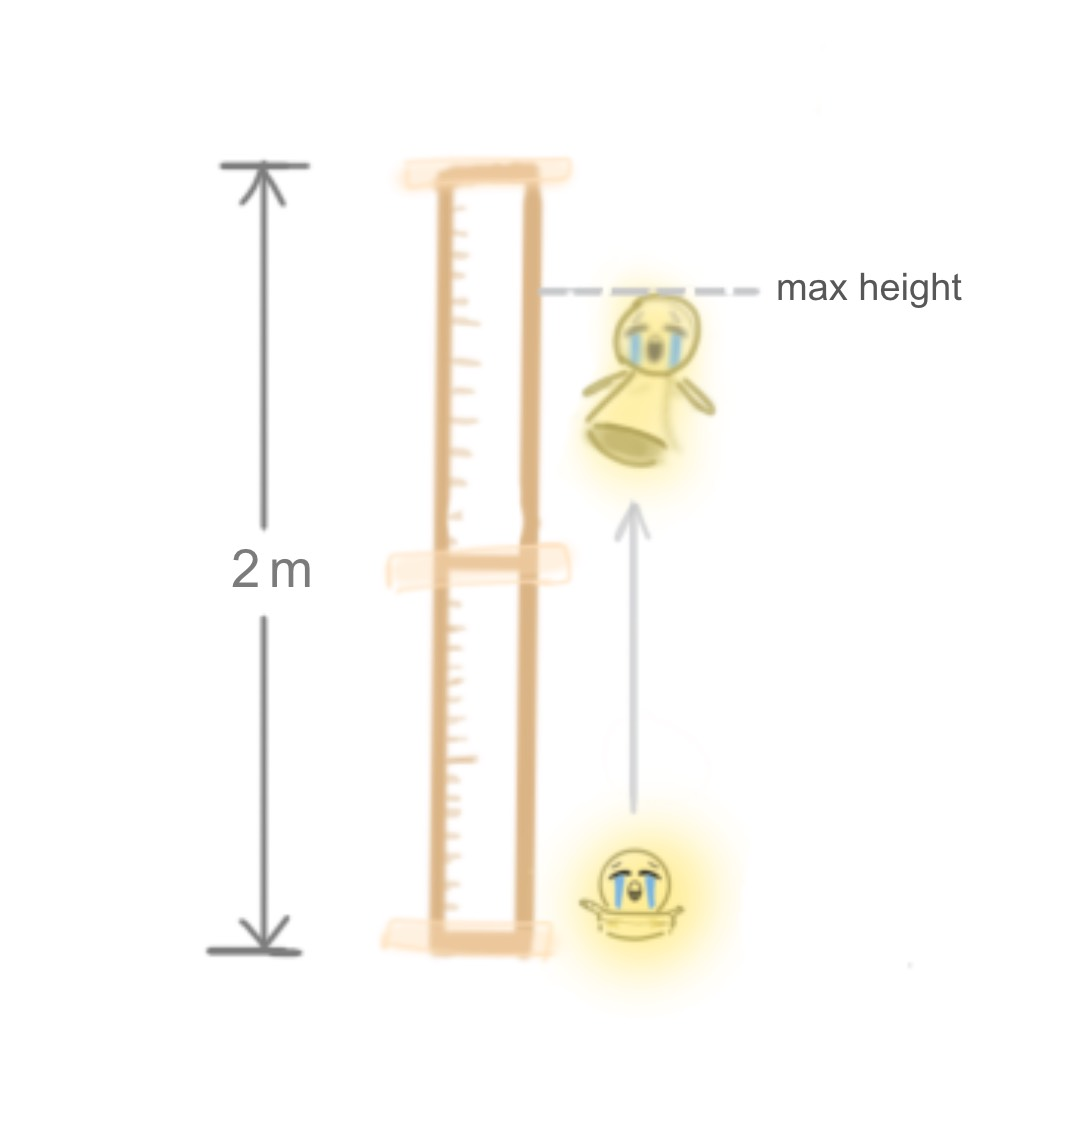
\includegraphics[width=0.5\textwidth]{figures/setupphoto.png} 
\caption{Experimental setup showing the vertical calibration scale and popper placement.}
\label{fig:setup}
\end{figure}
\section{Results}
The measured mass, maximum jump height, and calculated gravitational potential energy (GPE) for the ``happy'' and ``sad'' popper groups are summarized in \cref{tab:happy} and \cref{tab:sad}, respectively. 

\begin{table}[ht]
\caption{Mass, height, and potential energy for Happy Poppers.}
\label{tab:happy}
\begin{ruledtabular}
\begin{tabular}{cccc}
Trial & Mass (\unit{\kilo\gram}) & Height (\unit{\meter}) & GPE (\unit{\milli\joule}) \\
\colrule
1 & 0.0058 & 2.12 & 120.5 \\
2 & 0.0057 & 1.82 & 101.7 \\
3 & 0.0056 & 1.47 & 80.8 \\
4 & 0.0057 & 1.67 & 93.4 \\
5 & 0.0056 & 1.54 & 84.6 \\
\colrule
Mean & \num{0.0057} & \num{1.72} & \num{96.2} \\
Std. Dev. & \num{0.00008} & \num{0.26} & \num{15.6} \\
\end{tabular}
\end{ruledtabular}
\end{table}

\begin{table}[ht]
\caption{Mass, height, and potential energy for Sad Poppers.}
\label{tab:sad}
\begin{ruledtabular}
\begin{tabular}{cccc}
Trial & Mass (\unit{\kilo\gram}) & Height (\unit{\meter}) & GPE (\unit{\milli\joule}) \\
\colrule
1 & 0.0050 & 1.63 & 79.9 \\
2 & 0.0055 & 1.30 & 70.1 \\
3 & 0.0056 & 1.53 & 84.0 \\
4 & 0.0057 & 1.72 & 96.2 \\
5 & 0.0055 & 1.58 & 85.2 \\
\colrule
Mean & \num{0.0055} & \num{1.55} & \num{83.1} \\
Std. Dev. & \num{0.0002} & \num{0.16} & \num{9.2} \\
\end{tabular}
\end{ruledtabular}
\end{table}

The results of the two-sample $t$-tests are presented in \cref{tab:stats}. At the $\alpha = 0.05$ significance level, no statistically significant differences were found between the two groups for any of the measured variables.

\begin{table}[ht]
\caption{Two-sample $t$-test results for Mass, Height, and GPE.}
\label{tab:stats}
\begin{ruledtabular}
\begin{tabular}{lcccc}
Variable & $t$-value & $df$ & $p$-value & $\alpha$ \\
\colrule
Mass   & 1.74 & 8 & 0.12 & 0.05 \\
Height & 1.27 & 8 & 0.24 & 0.05 \\
GPE    & 1.62 & 8 & 0.15 & 0.05 \\
\end{tabular}
\end{ruledtabular}
\end{table}

\begin{figure}[ht]
\begin{center}
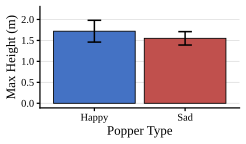
\includegraphics[width=0.45\textwidth]{figures/myplot.png}
\end{center}
\caption{Mean maximum jump height for happy and sad poppers. Error bars represent $\pm 1$ standard deviation ($n = 5$ per group).}
\label{fig:height_graph}
\end{figure}
\section{Discussion}
The results of this experiment indicate that popper design does not have a statistically significant effect on maximum jump height. Although the mean height of the happy poppers (\qty{1.72}{\meter}) was slightly greater than that of the sad poppers (\qty{1.55}{\meter}), the distributions overlap substantially, as indicated by \cref{fig:height_graph}. The two-tailed $t$-test gave a $p$-value of $0.24$, which is greater than $\alpha=0.05$. Therefore, we fail to reject the null hypothesis, indicating that facial expression does not significantly affect jump height. 

To better analyze the physics of the situation, GPE was calculated for each trial as well, as seen in \cref{tab:happy} and \cref{tab:sad}. Through this calculation, we were able to observe the transfer of elastic energy, from the popper being compressed, to motion (kinetic energy), to height. 

The calculated mean GPE values, seen in \cref{tab:happy} and \cref{tab:sad}, show a slight difference of \qty{13.1}{\milli\joule}. However, as seen in \cref{tab:stats}, a $t$-test between the two energy values resulted in $p=0.15 > 0.05$, indicating that the difference is not statistically significant and likely due to random variation. Since mass influences the conversion of energy into vertical motion, seen by \cref{eq:epe,eq:ke}, a statistical comparison of popper masses was performed. The comparison showed no statistically significant difference, with $p=0.12 > 0.05$, indicating that mass was likely not a confounding variable in the height comparison. 

The motion of the poppers is consistent with qualitative expectations from energy conservation. As illustrated by the experimental setup in \cref{fig:setup}, compressing the popper requires work to be done on the material, storing elastic potential energy. Upon release, this energy is converted into kinetic energy and then into gravitational potential energy at the peak of the jump. Although mechanical energy is not perfectly conserved due to non-conservative forces such as air resistance, sound, and internal deformation of the rubber, both popper types experienced similar conditions throughout the experiment. The comparable height distributions observed in \cref{fig:height_graph} therefore suggest that differences in facial design do not meaningfully affect the efficiency of energy transfer.

Overall, the statistical results and graphical evidence collectively support the hypothesis that facial expression does not influence maximum jump height. Instead, the motion of the poppers is governed primarily by elastic properties, mass and energy conservation and transfer mechanisms, rather than surface-level design features.

\subsection{Source of Experimental Error}
A possible source of experimental error is the force at which each popper is launched. Despite the fixed location, since each jumper was popped by one individual and not a repeatable machine, the angle, speed, pressure, and force that each jumper is pressed on can differ each time, causing variability in the data. Variability could also have been caused by error in human reaction. From the videos of each popper, the max height was analyzed. Humans can misread exact measurements on a meter stick, which could cause inconsistencies in data. Finally, the most likely cause of error is wear. As the poppers were used before, it is likely that there were internal deformations that may have led to inconsistencies within the data.

\section{Acknowledgements}
K. Coulanges, S. Dakwale, and S. Hein primarily led on data collection and recording. S. Hein compressed all the poppers to be released and wrote the abstract. S. Yellapragada wrote the introduction, methods and materials, R code for the graph, and revised the entire lab manuscript. R. Wallace calculated results based on height data. S. Dakwale explained sources of experimental error and performed all statistical analyses. K. Coulanges created setup figures and wrote the discussion. All members contributed to proofreading and editing, as well as feedback on the overall paper. We would like to thank Dr. Evangelista for providing guidance, materials, and supervision throughout the lab.

\bibliography{example.bib}
\end{document}
